\label{sec:empirical}
% Empirical	Approach
% Description of the empirical model: specification and variables involved
% Strategy for the estimation of the parameters of interest and test of the hypothesis
\subsection{Network Characteristics}
We start by characterizing the network. Recall, that we view airports as nodes, and flights between airports as edges. Considering the dataset of flights in 2018 from the Bureau of Transportation Statistics, we produce a network of US airports and the flights connecting them. We will refer to this network as the US Network. This network has 358 nodes and 3220 edges. With 310 nodes, the maximum possible number of edges would be (\cite{Barabasi Networks}): 
\begin{align}
    L_{max}  = \frac{N\cdot(N-1)}{2}=\frac{358\cdot(358-1)}{2} = 63.903
\end{align}
This implies, that only approximately 5 pct. of possible edges are actually found in the network. 
% Tjek nedenstående når vi ved mere
This sparseness of the network seems to support the hub-and-spoke nature of air transport; rather than having all airports be connected, it is more economically sensible to have certain airports function as hubs in their geographical area, and connect to hubs in other regional areas. \\ 
To get a further sense of how the network is connected we calculate the degree centrality for each node in the network, that is the number of other airports each airport is connected to through flights in 2018. \\
The average degree for the 358 airports contained in the dataset is 18,0. This average masks a huge variation; the highest degree found in the dataset is the O'Hare International Airport (ORD) in Chigago with a degree of 176.  Conversely, 51 airports have a degree of 1, implying that in this dataset they only appear in connection with a single other airport. \\
The degree distribution can be seen in the figure below. Clearly, a large number of airports are connected by flights to few other airports, while a minority of airports are much more connected.
\begin{figure}[H]
  \centering
  \caption{Domestic flights network, 2007}
    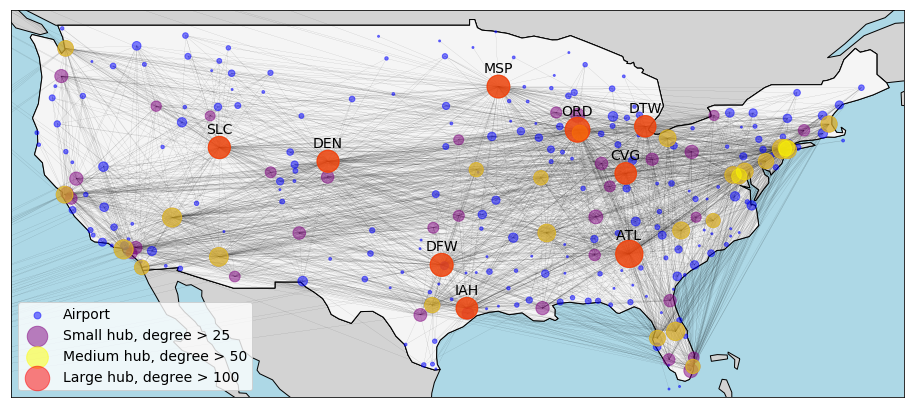
\includegraphics[width=1. \textwidth]{Exam/Figures/map_general_07}
    \vspace{-0.7cm}
    %\notecenter{Size resembles the degree.}
  \label{fig:map_general_07}
\end{figure}
\begin{figure}[H]
  \centering
  \caption{Domestic flights network, 2018}
    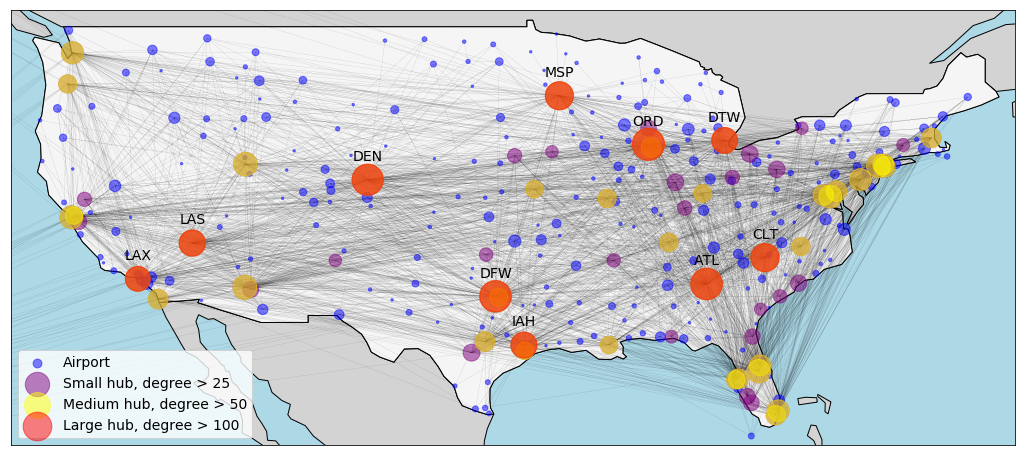
\includegraphics[width=1. \textwidth]{Exam/Figures/map_general_18}
    \vspace{-0.7cm}
    %\notecenter{Size resembles the degree.}
  \label{fig:map_general_18}
\end{figure}
As an alternative measures of centrality in the network, we calculate \textit{betweenness centrality} that measures the degree to which an edge is part of the shortest path between two other edges where path length is defined as the number of traversed links. \\
In the end, we use clustering coefficient, betweenness and degree as features in the prediction model. Note, that these are all node-specific measures, and as such, for each observation, there are two of each corresponding to origin and destination airport. 

% Figur med hhv. degree distribution (til venstre) og betweenness centrality (højre)?
The figure below shows every airport in the network we consider, and the edges that connect them. The network is distributed spatially according to the actual geographical locations of the airports, and overlaid on a map of the continental US. From a visual examination the hub-and-spoke nature of the network becomes clear.

The figure below shows the degree distribution of the network. The hub-and-spoke nature of the network - and the related fact that it is scale-free - is fairly apparent: A large number of nodes have a low degree, while a few nodes have a degree far above the average degree. 
\begin{figure}[H]
  \centering
  \caption{Degree distribution of network, 2018}
    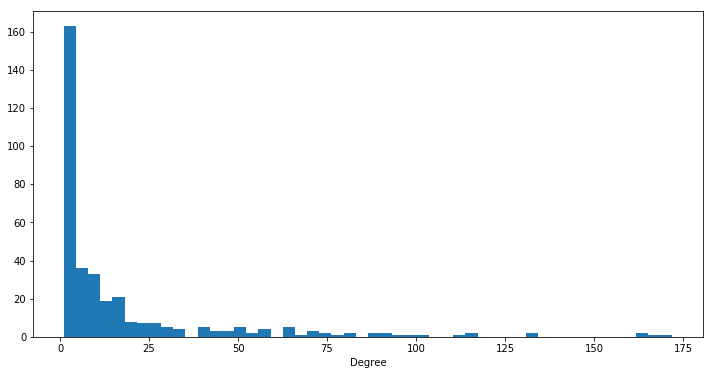
\includegraphics[width=0.6 \textwidth]{Exam/Figures/degreeDistribution.png}
  \label{fig:degreeDistribution}
\end{figure}
Similar figures for betweenness centrality and clustering coefficient can be found in figure \ref{fig:Btwns_CC} in appendix \ref{app: Network characteristics}. 

\subsection{Network vulnerability}
We conduct an analysis of how the network is affected when certain nodes are removed. This analysis is, broadly, in line with the analysis in \cite{chi2004structural}. \\
The figure below shows how key network characteristics (average degree, clustering coefficient and global efficiency) are affected, when nodes are removed. One curve corresponds to removal of the most connected nodes, this is what we refer to as an 'attack' on the network, where the hubs are targeted. \\
Secondly, we consider how the network is affected when we remove the least important nodes first. \\
Finally, we consider how the network is affected by an event that removes all network in a geographical area (such as might be the case due to natural disaster og extreme weather conditions). We conduct this analysis by choosing a spot in the continental US, calculating the (geographical) distances from each airport to this spot, and then removing all airports within x miles. This final analysis takes advantage of the spatial nature of the network, and provides insight into how geographically determined failures may affect the network. \\
It should be noted, that in this section we analyze the network as it is in our dataset. Obviously, were a number of airports to close for a prolonged period (e.g. due to natural disaster), the agents in the market would make changes to the network to accommodate the new situation. Market forces is likely to have been a determinant in producing the network as is, and exogenous changes to the network would cause changes in behaviour of the agents in the market, that would produce a new network. \\ 

\begin{figure}[H]
  \centering
  \caption{Effect of node removal on average degree (left) and clustering coefficient (right)}
    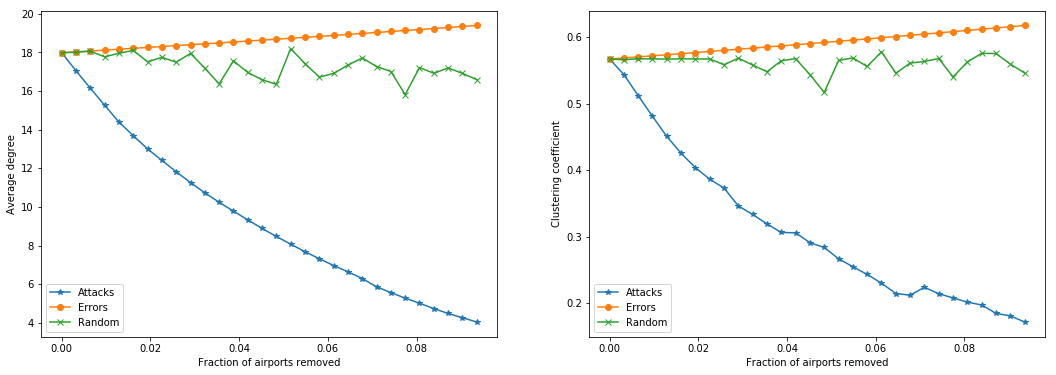
\includegraphics[width=1. \textwidth]{Exam/Figures/attacksanderrors.png}
  \label{fig:attacks_and_errors}
\end{figure}
As the figure shows, the removal of a relatively small number of hubs can dramatically alter network characteristics. Unsurprisingly, removal of the least important nodes increases the measures. The network is thus somewhat vulnerable to 'attacks' on the most connected airports. \\ In the figure, we also show the effect of removing random nodes. Note, that each point represents a "new" network of randomly chosen nodes in the original network. Nodes left out in the first observation may therefore be present in the second observation.  Removal of random nodes has relatively little effect on average degree or the clustering coefficient of the network, again pointing to the fact that the network is vulnerable only to a concerted attack on important hubs. \\ 

\subsection{Predicting Flight Prices - Do Network-related Features add Predictive Power?}
Our set of network-related features includes, for both origin and destination airport: Betweenness centrality, degree and clustering coefficient. \\
Our set of other features includes: The number of flights on the given route in the year considered, the distance between the two airports, the (average) time in minutes for the flight and the number of carriers who flew the route during the year considered. \\

\begin{figure}[H]
  \centering
  \caption{Correlation plot, 2007}
    
\includegraphics[width=1. \textwidth]{Exam/Figures/corr_plot.pdf}
  \label{fig:map_general}
\end{figure}
Our key question is then whether or not adding the network-related features contributes predictive power in predicting prices. 

In order to predict prices we use a linear prediction model including network characteristics and distance as predictors.

We write our prediction model as
$$
p_i = w_0 + W X_i 
$$
where $p_i$ is the price of a given flight, $w_0$ is the bias/intercept, $X_i$ is a vector of predictors, and $W$ is a vector of corresponding weights. 

To find the weights that makes the most accurate predictions we need to define a cost function. The standard cost function estimating a linear model is the \textbf{Mean Squared Error (MSE)}:
$$
\text{MSE}=\frac{1}{N} \sum_i^N (y_i - (w_i + WX_i)^2
$$
However, we allow for a more flexible cost function called using estimation method called elastic net which incorporates both the LASSO and the RIDGE regularization in the objective function. 

The best model is found using Cross Validated Grid Search from SKLEARN module in Python. We search for 